%to have line numbers
%\RequirePackage{lineno}
\documentclass[10pt, letterpaper]{article}      
\usepackage[margin=.1cm,font=small,labelfont=bf]{caption}[2007/03/09]
%\usepackage{endnotes}
%\let\footnote=\endnote
\usepackage{setspace}
\usepackage{longtable}                        
\usepackage{anysize}                          
\usepackage{natbib}                           
%\bibpunct{(}{)}{,}{a}{,}{,}                   
\bibpunct{(}{)}{,}{a}{}{,}                   
\usepackage{amsmath}
\usepackage[% draft,
pdftex]{graphicx} %draft is a way to exclude figures                
\usepackage{epstopdf}
\usepackage{hyperref}                             % For creating hyperlinks in cross references
\hypersetup{pdfborder={0 0 0.4}} %have nice light boxes on refs

% \usepackage[margins]{trackchanges}

% \note[editor]{The note}
% \annote[editor]{Text to annotate}{The note}
%    \add[editor]{Text to add}
% \remove[editor]{Text to remove}
% \change[editor]{Text to remove}{Text to add}

%TODO make it more standard before submission: \marginsize{2cm}{2cm}{1cm}{1cm}
\marginsize{1cm}{1cm}{.5cm}{.5cm}%{left}{right}{top}{bottom}   
					          % Helps LaTeX put figures where YOU want
 \renewcommand{\topfraction}{1}	                  % 90% of page top can be a float
 \renewcommand{\bottomfraction}{1}	          % 90% of page bottom can be a float
 \renewcommand{\textfraction}{0.0}	          % only 10% of page must to be text

 \usepackage{float}                               %latex will not complain to include float after float

\usepackage[table]{xcolor}                        %for table shading
\definecolor{gray90}{gray}{0.90}
\definecolor{orange}{RGB}{255,128,0}

\renewcommand\arraystretch{.9}                    %for spacing of arrays like tabular

%-------------------- my commands -----------------------------------------
\newenvironment{ig}[1]{
\begin{center}
 %\includegraphics[height=5.0in]{#1} 
 \includegraphics[height=3.3in]{#1} 
\end{center}}

 \newcommand{\cc}[1]{
\hspace{-.13in}$\bullet$\marginpar{\begin{spacing}{.6}\begin{footnotesize}\color{blue}{#1}\end{footnotesize}\end{spacing}}
\hspace{-.13in} }

%-------------------- END my commands -----------------------------------------



%-------------------- extra options -----------------------------------------

%%%%%%%%%%%%%
% footnotes %
%%%%%%%%%%%%%

%\long\def\symbolfootnote[#1]#2{\begingroup% %these can be used to make footnote  nonnumeric asterick, dagger etc
%\def\thefootnote{\fnsymbol{footnote}}\footnote[#1]{#2}\endgroup}	%see: http://help-csli.stanford.edu/tex/latex-footnotes.shtml

%%%%%%%%%%%
% spacing %
%%%%%%%%%%%

% \abovecaptionskip: space above caption
% \belowcaptionskip: space below caption
%\oddsidemargin 0cm
%\evensidemargin 0cm

%%%%%%%%%
% style %
%%%%%%%%%

%\pagestyle{myheadings}         % Option to put page headers
                               % Needed \documentclass[a4paper,twoside]{article}
%\markboth{{\small\it Politics and Life Satisfaction }}
%{{\small\it Adam Okulicz-Kozaryn} }

%\headsep 1.5cm
% \pagestyle{empty}			% no page numbers
% \parindent  15.mm			% indent paragraph by this much
% \parskip     2.mm			% space between paragraphs
% \mathindent 20.mm			% indent math equations by this much

%%%%%%%%%%%%%%%%%%
% extra packages %
%%%%%%%%%%%%%%%%%%

\usepackage{datetime}


\usepackage[latin1]{inputenc}
\usepackage{tikz}
\usetikzlibrary{shapes,arrows,backgrounds}


%\usepackage{color}					% For creating coloured text and background
%\usepackage{float}
\usepackage{subfig}                                     % for combined figures

\renewcommand{\ss}[1]{{\colorbox{blue}{\bf \color{white}{#1}}}}
\newcommand{\ee}[1]{\endnote{\vspace{-.10in}\begin{spacing}{1.0}{\normalsize #1}\end{spacing}\vspace{.20in}}}
\newcommand{\emd}[1]{\ExecuteMetaData[/tmp/tex]{#1}} % grab numbers  from stata

%TODO before submitting comment this out to get 'regular fornt'
\usepackage{sectsty}
\allsectionsfont{\normalfont\sffamily}
\usepackage{sectsty}
\allsectionsfont{\normalfont\sffamily}
\renewcommand\familydefault{\sfdefault}

%\usepackage[margins]{trackchanges}
\usepackage{rotating}
\usepackage{catchfilebetweentags}

\usepackage{abstract}
\renewcommand{\abstractname}{}    % clear the title
\renewcommand{\absnamepos}{empty} % originally center
%-------------------- END extra options -----------------------------------------
\date{{}\today \hspace{.2in}\xxivtime}
\title{  % remember to have Vistula University!!
  Hey! Cities! Leave Them Kids Alone!\footnote{The title paraphrizes the classic Pink
    Floyd's song: \url{https://www.youtube.com/watch?v=qs35t2xFqdU}} \\
  \Large{(Urban Adolescents Have Lower Life Satisfaction and Eudaimonia)} % than rural ones %(urban unhappiness is common in adolescents)
}
\author{
% Adam Okulicz-Kozaryn\thanks{EMAIL: adam.okulicz.kozaryn@gmail.com
%   \hfill I thank XXX.  All mistakes are mine.} \\
% {\small Rutgers - Camden  % and Vistula University
% }
}

\begin{document}

%%\setpagewiselinenumbers
%\modulolinenumbers[1]
%\linenumbers

\bibliographystyle{/home/aok/papers/root/tex/ecta}
\maketitle
\vspace{-.4in}
\begin{center}

\end{center}


\begin{abstract}
  \noindent This is the first study to focus on the urban-rural happiness gradient
  in adolescents. Using the 2018 Programme for International Student Assessment
  (PISA) dataset of about .5m adolescents, we  find a moderately large negative effect of large city ($>$1m) on
  happiness: about -0.5 on a 0-10 scale, and for some countries a larger effect, close to -1.   % shows no significant relationship, and 2 out of 71 show positive effect.
  We explore not just cognitive life satisfaction, but also the relatively rarely studied
  Eudaimonia, which reveals a similar urban-rural gradient. By studying
  adolescents, we mitigate self-sorting issues since adolescents, in general, do
  not move by choice. 
  % Still, causality may not be present as in any non-experimental study.
  We address another potential source of sorting (due to parental choices) by
  comparing the urban-rural gradient for adolescents with that typically found
  for adults.
\end{abstract}
\vspace{.15in} 
\noindent{\sc Programme for International Student Assessment (PISA), happiness,
  life satisfaction, subjective wellbeing, urban-rural, cities} 
\vspace{.25in} 

\begin{spacing}{1.4} %TODO MAYBE before submission can make it like 2.0
\rowcolors{1}{white}{gray90}

\textbf{Highlights}

\begin{itemize}
\item first study to focus on urban-rural happiness gradient in adolescents
\item moderate effect  of large city ($>$1m) on happiness: about -0.5 on
  0-10 scale
\item negative effect  of large city ($>$1m) also on eudaimonia: -.1 to -.15 on % -2.1 to 1.7
 on a standardized scale
\end{itemize}

%  instead \ExecuteMetaData[../out/tex]{ginipov} do \emd{ginipov}

% \begin{figure}[H]
%  \includegraphics[height=3in]{../out/gov_res_trust.pdf}\centering\label{gov_res_trust}
% \caption{woo}
% \end{figure}


%TODO !!!! have input here aok_var_des

\noindent 

When asking a parent what they want most for their children, many would arguably
respond, ``I want them to be happy.'' Parents typically wish that their kids
will find fulfillment and happiness in life, and most worry about their kids'
mental health and well-being. A recent survey from the Pew Research Center found
that 40\% of parents were extremely, or very worried, about their children
struggling with anxiety or depression \citep{pew}. Mental health issues among
adolescents are on the rise, with rates of depression and anxiety among
teenagers increasing at a faster rate than in adults \citep{cdc}. The COVID
pandemic  played a role in this trend, but there are many other factors that can
affect a teen's mental health such as interaction with friends, isolation,
school environment and parent's relationship \citep{twenge12,twenge14,twenge15,twengeATL17sep}. 

We explore how the place in which adolescents live can be related to their
well-being and sense of happiness. Although happiness may not be the sole goal
for adults,\footnote{Some adults may have as their primary goal duty, service, work, doing the
  right thing, and so forth, and in doing so they may actually forego happiness
  for something else.} happiness is what most parents want for their children, and what many young people desire \citep{humphrey2023}. Furthermore, wellbeing in childhood is positively related to the child's future adult
 wellbeing, even after controlling for family and other influences
 \citep{de2012estimating}. 
 

To achieve greater happiness, should adolescents experience more urbanity or more rurality? Findings should be of interest to policymakers, administrators, schools, and 
parents. Adults tend to be less happy in cities across the world
(except in the poorest regions such as Sub-Saharan Africa and parts of Latin
America \citep{aok21,valente2016}, but we know little about how living in an
urban versus rural area can affect the wellbeing of adolescents
\citep{marquez24}, with evidence especially missing about eudaimonia (self-assessed meaning in life).  

Thus, to address these issues,  we conduct quantitative analyses that explore how
urbanicity can affect adolescents'  wellbeing (both life satisfaction and
eudaimonia). The paper is structured as follows: we start by exploring the
literature on child and adolescent wellbeing. Next, we examine the theory and
mechanisms driving urban vs. rural happiness. % : remarkably, there is no
% quantitative study exploring how urbanicity affects teens.
Our data and
empirical analysis follows and we conclude with a discussion of results and
takeaways for policy and practice.


\section*{Child and Adolescent  Wellbeing Literature}



According to Bronfenbrenner's bioecological systems model
\citep{bronfenbrenner2007}, children's and adolescents' wellbeing is affected by
their surroundings at different scales. Most immediately, their wellbeing is
affected by their parents' wellbeing, which may reflect the parents' mental
states and/or their overall life satisfaction. At a broader scale, the child's
wellbeing may be affected by their living environment including the immediate
neighborhood and where they live on an urban-rural spectrum. 
 %
 For instance, in developing countries, 
overcrowding and environmental pollution are massive urban problems made worse by
undernutrition and infections, particularly respiratory and diarrhoeal
diseases. In developed societies there are many other urban problems, e.g., injuries,
poisonings, violence, drug abuse, exposure to industrial and atmospheric
pollutants, including pesticides, sexually transmissible diseases, and
``lifestyle'' diseases including obesity and cardiovascular disease risk \citep{gracey2002child}.
% \citet{gracey2002child} provides an useful overview of effects of urbanization
% on children, which is summarized in this paragraph. In developing countries,
% overcrowding and environmental pollution are massive problems made worse by
% undernutrition and infections, particularly respiratory and diarrhoeal
% diseases. In developed societies there are many other problems, e.g. injuries,
% poisonings, violence, drug abuse, exposure to industrial and atmospheric
% pollutants, including pesticides, sexually transmissible diseases, and
% ``lifestyle,'' diseases including obesity and cardiovascular disease risk.
At each scale, effects may be gender-specific, especially for adolescents. For
instance, \citet{nolen2016} find that depression is more common amongst female
adolescents than amongst males of the same age.

The relationship of parents' wellbeing with child and adolescent wellbeing has
been examined across diverse settings with somewhat conflicting
results. \citet{powdthavee2008}, using British longitudinal data (BHPS), find that the
father's mental distress predicts subsequent life satisfaction both of
adolescent boys and girls, while mother's mental distress predicts subsequent
life satisfaction of adolescent girls but not of boys. Analyses using the same
BHPS data source also indicate a positive relationship between parent and child
life satisfaction \citep{clair2012relationship} and there is also a long-term
(20 year) impact of the mother's mental health on the subsequent subjective
wellbeing of their children \citep{layard2014,clark2019}. Results using US data
(from the Fragile Families Longitudinal Survey which primarily has an urban
sample) reveal that higher parental wellbeing spills over to positive subjective
wellbeing for adolescents \citep{coles2022,park2024}.
 %
However, \citet{bedin2014dyadic}  find that such spillover effects are small in
their study of parent-adolescent dyads in Brazil. Similarly,
\citet{casas2008does, casas2012testing}  find only a very weak relationship between parents' and their
adolescents' wellbeing, especially for their male offspring.

\citet{bryant2018} find in Australia that children of refugee parents with PTSD
have greater emotional problems than children of refugees who do not suffer from
PTSD. Within developing countries, \citet{borga2022} find a strong correlation
between parent and child wellbeing when using longitudinal data from Ethiopia,
India, Peru and Vietnam. Their analysis, however,  attributes this correlation to the impact of the shared environment, rather than being due to specific parental attributes. When splitting the analysis between rural and urban samples, the study finds that mother's health is correlated with child subjective wellbeing in rural areas but not in urban areas.
Other than the \citet{borga2022} study, only a few studies have examined child
wellbeing in urban relative to rural or remote areas. Some studies find that
child (and especially adolescent) wellbeing is lower in rural or remote areas
than in urban areas; however, these studies tend to cover only limited areas. For example in the case of Scotland, \citet{levin2014} finds some evidence that, relative to urban areas, adolescent mental health is lower in remote rural areas than in urban areas while life satisfaction is lower in accessible rural areas; other wellbeing measures show no difference across the urban/rural divide. Similarly, \citet{parkes2016} find that remote location predicted poorer wellbeing outcomes for 7 year old children in Scotland, even after controlling for other factors. For Turkey, \citet{yeresyan2014} find lower wellbeing of adolescents in rural than in urban areas but find no such relationship for adolescents in Germany. 
The effects on wellbeing of living in a rural versus urban area may differ by
gender. \citet{powdthavee2008} discuss the possibility that adolescents' need
for friends and other close relationships may be greater for females than for
males. They do not test whether this explanation may lead to gendered outcomes
in urban versus rural locations; however, if their hypothesis is correct then it
may be the case that the gender wellbeing divide differs across rural versus
urban areas; subsequently, we test for such an effect.

The nature of the surrounding environment may also impact child (and adult) wellbeing. Within the US, \citet{fava2022} find that a better neighborhood perception by the mother when the child is 3 years old is associated with higher child wellbeing when the child is 9 years old. Using data from urban Catalonia, \citet{oriol2023} find that the degree of optimism of an adolescent (and a child) is positively related to their subsequent cognitive and affective wellbeing. If optimism is determined in part by the surrounding community, and not just by personal and parental characteristics, then the nature of the community that one lives in may also be influential for adolescent and child wellbeing through this channel. 
%RV: Make sure the marquez24 citation is correct on bibtex, should just be Marquez (2017), without the J. 
Using a related dataset to ours, \citet{marquez24} find that adolescent life satisfaction is positively
related to family wealth and is decreasing in the size of
settlement. \citet{marquez24} does not focus on urban-rural differences,
however, but instead focuses on global trends in adolescent wellbeing.  
 \citet{marquez24} uses 2022 OECD PISA (Programme for
International Student Assessment) data which is available for 74 countries (although regression results are
presented for respondents only from 43 countries).\footnote{A second model, estimated for respondents in 13 countries, includes a range of controls
  for satisfaction with local services and environment.}
While the study controls for country GNI per capita, it does
not include country fixed effects to control for other factors (e.g., national cultural differences). Furthermore,
the use of 2022 data leaves open the possibility that the results are affected by the differential impact of COVID
and related policy responses across settlement types.
 %new edits by rubia
Our study, which uses 2018 PISA data pre-dates these COVID effects.

In addition,
we examine the relationship not just of settlement size to life satisfaction but
also to eudaimonia which has not been examined for adolescents across
urbanicity. Additionally, we test if effects differ between males and
females. Even though the evidence is not unanimous, some aspects of adolescent
wellbeing are likely to be influenced by parents' mental states though the
effects may be small and are likely to be gendered. Studies are less unanimous
on whether an urban/rural divide in wellbeing exists for adolescents, and
whether any such divide (if it exists) differs between boys and girls.

For adults,  \citet{aok11a} confirmed that at least in the
US, there's a gradient in SWB that rises from its lowest levels in the large
cities to its highest levels in the rural periphery, the so called ``urban-rural
happiness gradient,'' when controlling for many of the characteristics that
affect individual' happiness. In our own testing, while we cannot control for
parents' wellbeing, we do control for material wellbeing of the family, which is
a major determinant of adult subjective wellbeing \citep{clark2018}. Controlling for
this factor (and others) we test whether adolescents face an urban/rural divide
in wellbeing, and whether an urban-rural gradient is present for adolescents,
measured by both life satisfaction and eudaimonia. In addition, we test whether
these results are consistent across adolescent boys and girls.




\section*{Theory and Mechanisms of Urban Unhappiness}

% rephraze copied from swbUrbRurPsid
 Genes determine about half of subjective wellbeing (SWB)
 \citep{schnittker08,lykken96t,brooksGenetic}.
 %
 %
 Humans have not
evolved for city life---living in an artificial setting among thousands of people densely packed together. Some animals such as ants or bees may thrive in a high density environment, but not humans: for over 95\% of our evolutionary history there were no cities---hunters and
gatherers lived in bands of 50-80 people \citep{maryanski92}. Humans evolved to
prefer nature and those who learned how to live in harmony with nature are more
likely to survive and thrive \citep{pretty12,yamamoto16}. 
%Humans have evolved to prefer and be happy in nature,  open space
%there was that citation that i have recently seen but forgot where that that
%humans evolved to prefer nature--those who prefered it and were in harmony with
%it were more likely to survive etc
Concurrently, a defining feature of cities is heterogeneity or diversity \citep{wirth38}, which accordingly produces: 
 mistrust, uneasiness, conflict, and misanthropy
 \citep{milgram70,thrift05,amin06,aok22}.\footnote{Yet, on the other hand, at least in theory, in a city there can be community: for example, a neighborhood village, that at least in some ways can simulate a more natural habitat for humans \citep{fischer95,fischer75,jacobs93}.}
Ingroup preference or homophily (love of the same) theory explains this process: humans have preference for other humans who they perceive to be ``like them'' \citep{mcpherson01,tajfel82,tajfel71,smelser99,putnam07,christakis09f}, and dislike outgroups or dissimilar persons. Therefore, living in a densely populated heterogeneous place can contribute to unhappiness.


Livability theory \citep{veenhoven95,veenhoven14b,veenhoven00b} states that humans, just like other animals, have needs (such as those on the Maslow's Hierarchy of Needs \citep{maslow87}), and if those needs are satisfied, then conditions are livable, and happiness follows. 
However, it is unclear what the livability theory predicts in regards to urbanism. Some aspects of city life may improve livability, and hence, happiness. Cities have multiple benefits  \citep{meyer13,florida08,glaeser11,osullivan09}, notably jobs and amenities that improve livability and
 happiness. But cities also  have multiple problems such as congestion, high
 rates of crime, rapid spread of infectious diseases, air, noise, and light
 pollution 
   \citep{bettencourt10b,bettencourt07,meyer13,aokCityBook15,aok21}.
   % \footnote{Measuring
     % it with happiness yardstick,  city disadvantages outweigh city
     % advantages--cities are less happy (at least in the developed world)
     % \citep{aok21}.}
    %
And these problems can be  exacerbated among children and adolescents, who are
more vulnerable than adults. For example, urban crime (and bullying) is arguably
more of an issue for adolescents (perhaps especially females) than for adults
who may be better able to insulate themselves from it\footnote{Adults usually
  spend most of their  time at work, at home, or in a car, which are relatively
  crime free zones, whereas an adolescent is arguably less able to insulate
  herself from their neighborhood and peers. It is important to highlight that
  crime is a feature of cities, with crime increasing consistently with city size \citep{blissCL_nov4_14,bettencourt13,bettencourt10,bettencourt10b,bettencourt07}.}
 and cope with it. Indeed,  adults have better coping mechanisms than adolescents since coping increases with age \citep{leipold2019coping}. 

A century ago, \cite{simmel03} theoretized that urbanism has a negative effect on human brains and neural processing. Most recently, this finding was confirmed by neuroscience---even growing up in a city has lasting negative effects later in life \citep{lederbogen11}. 
   
Furthermore, the Multiple Discrepancies Theory (MDT)
\citep{michalos85,michalos14c} states that happiness is relative and a result of
multiple comparisons. Visual and social comparisons are more likely in urban
areas as there are more people and more stimuli. There is some evidence that
humans tend to make upwards comparisons \citep{frey02s} thus ending up feeling
relatively deprived \citep[e.g.,][]{luttmer05,frank12}. Adolescents, like
adults, are likely to want to keep up with the ``Joneses,''  e.g., through clothing, jewelry, parties, cars---see examples in \citet{frank12}. 
 
Similarly, as in adults,  there are other mechanisms that can impact
adolescents' happiness in cities. The denser the city, the less nature there is 
\citep{aokCityBook15} and nature is key for human flourishing \citep{pretty12}. Cities tend to be the most polluted places on Earth % (although they pollute least per capita)
\citep{meyer13}, and not just in terms of air pollution, but also light and
noise pollution, each of which can reduce happiness \citep{signoretta19,poonCL18jan29,leeTT16feb13,metcalfeCL16jun10,weinhold12,rehdanz08,welsch05,york03}. Materialism and consumerism (and unethical behavior) are also concentrated in cities \citep[e.g.,][]{aok-sizeFetish17,okulicz2022materialism,morris21,wirth38} and
 are likely to result in unhappiness particularly when focused on purchasing
 material goods and not experiences,  at the cost of human needs such as social connection
 \citep[e.g.,][]{frank12,leonard10,vanboven05,burroughs02,dumludag21}.\footnote{Also see \citet{wu20,wang17,brown19,brown17}.}
  
%On the other hand, the smaller the place, the more homegeneity, the more trust and higher levels of wellbeing \citep{putnam07,aok22,herbst14,vogt07}.
%RV: not sure this flows, so commented out for now

\citet{morrison2024resolving} tries to resolve the urban unhappiness paradox by
argiung that if there were more skilled workers in a city, cities would not be
less happy. It is a familiar argument by economists that more education solves
just about anything. While we agree that more skilled workers would make cites
less unhappy, there is a number of other mechanisms for urban unhappiness as
discussed above. \citet{morrison2024resolving} further argues other mechanisms. 
1) education  boost social engagement. Yet from anectodal experience
we see uneducated people most socially engaged and PhDs least. 2) cities promote
social interaction. Some forms, but most forms are inhibited by urbanism as
discussed above.
 
Studying urban vs. rural happiness among  adolescents has an advantage over adults. Some have argued that there may be self sorting of unhappy adults into cities, i.e., it is not that cities make people unhappy, but that unhappy people move to cities. For instance, ``Veenhoven (1994) argues that cities attract
those already dissatisfied with their life in rural areas, and hence there could
be an excess of unhappy/unsatisfied people in cities. For him, cities do not
make unhappy people but attract them''\citep[cited in][]{ebshoy24}. The issue of
reverse causality is mitigated when focusing on children and adolescents because
unlike adults, they do not self-sort or move into areas by
choice.\footnote{While it is true that adolescents cannot choose where they
  live, parents indeed make such a choice, so if happier parents choose to live
  in rural areas, and there is an intergenerational correlation in
  wellbeing, then it is hard to interpret a causal link from urbanicity to
  wellbeing in adolescents. While there is conflicting evidence as to the degree to which this
  intergenerational link exists, it is something to note nonetheless.}
Previous
research has partially explored this issue by using the US GSS survey item,
``Which of the categories on this card comes closest to the type of place you
were living in when you were 16 years old?'' \citep{aok20}. Growing up in urban
areas had a lasting negative effect on happiness among adults in the U.S. later
in life \citep{aok20}. We build on this body of research by asking actual
adolescents (15 years old) about their happiness and place of residence (instead
of asking adults to recall their adolescence), and we expand the research scope
by examining adolescents  over a wide range of countries, not just the United States. 


\section*{Data}

We use the 2018 PISA data % (Programme for International Student Assessment)
 from \url{oecd.org/pisa/data/2018database}. Respondents are adolescents (the vast majority are 15 year olds, and a few 16 year olds).
 %
The 2018 PISA is a large dataset with $>.5m$ observations across 80 %142
countries (including several sub-country regions), % \footnote{The adolescent datafile at \url{https://www.oecd.org/pisa/data/2018database} has 80 countries. PISA website lists 83 participants at \url{https://www.oecd.org/pisa/aboutpisa/pisa-participants.htm}.}
 and  has a wellbeing module with several subjective wellbeing (SWB) items. 

Urbanicity is recorded in school questionnaires administered to school
principals (an objective urbanicity measure)\footnote{Urbanicty of school and
  residence will be arguably highly correlated, but it is not the same. Arguably
  some smaller area dwellers may be counted as larger area as the school if not
  the same urbanicity will be rather in larger than smaller place as per central
  place theory.
}% , unlike Gallup World Poll \citep{aok21})
: ``Which of the following definitions best describes the community in which your school is located?''
\begin{itemize}
\item A village, hamlet or rural area (fewer than 3,000 people)
\item A small town (3,000 to about 15 000 people)
\item A town (15,000 to about 100,000 people)
\item A city (100,000 to about 1,000,000 people)
\item A large city (with over 1,000,000 people). 
\end{itemize}

The top bin (large city $>1m$) provides an advantage over the widely used World Values Survey, where the top urbanicity cutoff is only .5m \citep{deb23,ebshoy24}. Urbanicity is missing for only 5.5 percent of
observations. 

PISA uses the 0-10 life satisfaction measure: ``Overall, how satisfied are you with
your life as a whole these days?''
 This measure is similar to the Cantril ladder which has been shown to be a valid tool for
measuring the subjective wellbeing of 15 year-olds \citep{levin2014reliability}.
 %
 The life satisfaction measure is missing for several countries, thus the sample size is reduced from 80 to 72 countries---tables in the results section list the countries used in our analyses. 

The PISA 2018 dataset also contains a relatively rarely measured eudaimonic wellbeing variable \citep[see][]{proctor16}. PISA defines meaning in life as the extent to which 15-year-olds comprehend, make sense of, or find significance in their lives \citep{pisa18}. PISA 2018 asked students whether they agreed or disagreed (``strongly disagree,'' ``disagree,'' ``agree,'' ``strongly agree'') with the following
statements: ``My life has clear meaning or purpose;'' ``I have discovered a
satisfactory meaning in life;'' and ``I have a clear sense of what gives meaning
to my life.'' These statements were combined to create a standardized index (mean=0, standard deviation=1) of meaning in life, thus measuring eudaimonic wellbeing. 


Basic controls in our models are gender and family wealth (age, education, and
marital status are mostly constant and so are omitted). In addition, we control
for mother's education. Most work on children and adolescents finds that
mother's education is more important for children' health outcomes than father's
education \citep{nepal2018matters} and information for mothers is less likely to
be missing from surveys than is fathers' information (fathers are more often
missing than mothers from the household). 

 %
We also control for internet use on weekdays and weekends, and we utilize  specific measures of how the
internet is used outside of school (for  social media use and ``for fun''). This control is particularly important as  social media can
drastically reduce and impact happiness among the youth
\citep{twengeATL17sep,twenge14}, and could potentially be correlated with
urbanicity. All of the variables and controls used in our analyses are listed
in Table \ref{var_des}. Variables' distributions are in appendix.

There are data limitations. There are no measures of siblings
and grandparents, and we did not find a good health variable---existing ones are
missing for the vast majority of respondents. Health is of course a key
happiness predictor, but arguably less important for adolescents as they are
healthier than adults, and since age is constant, we expect there is less variability in
health for this age-group than for adults. These limitations aside, we  note
that PISA is a particularly rich data source  for urban/happiness researchers. PISA covers $80+$ countries with multiple waves going back to 2000, and large sample size of $500,000+$ with hundreds of variables. % It is currently underused, for instance, only 4 papers in the journal \textit{Cities} have used it, and all focusing on China only \citep{hu2019segregation,du2020influence,murgante2024developing,lee2022drives}. 
 
\input{varDesED.tex} 

\section*{Results}

%meh have plenty of tables
% \begin{figure}[H]
%  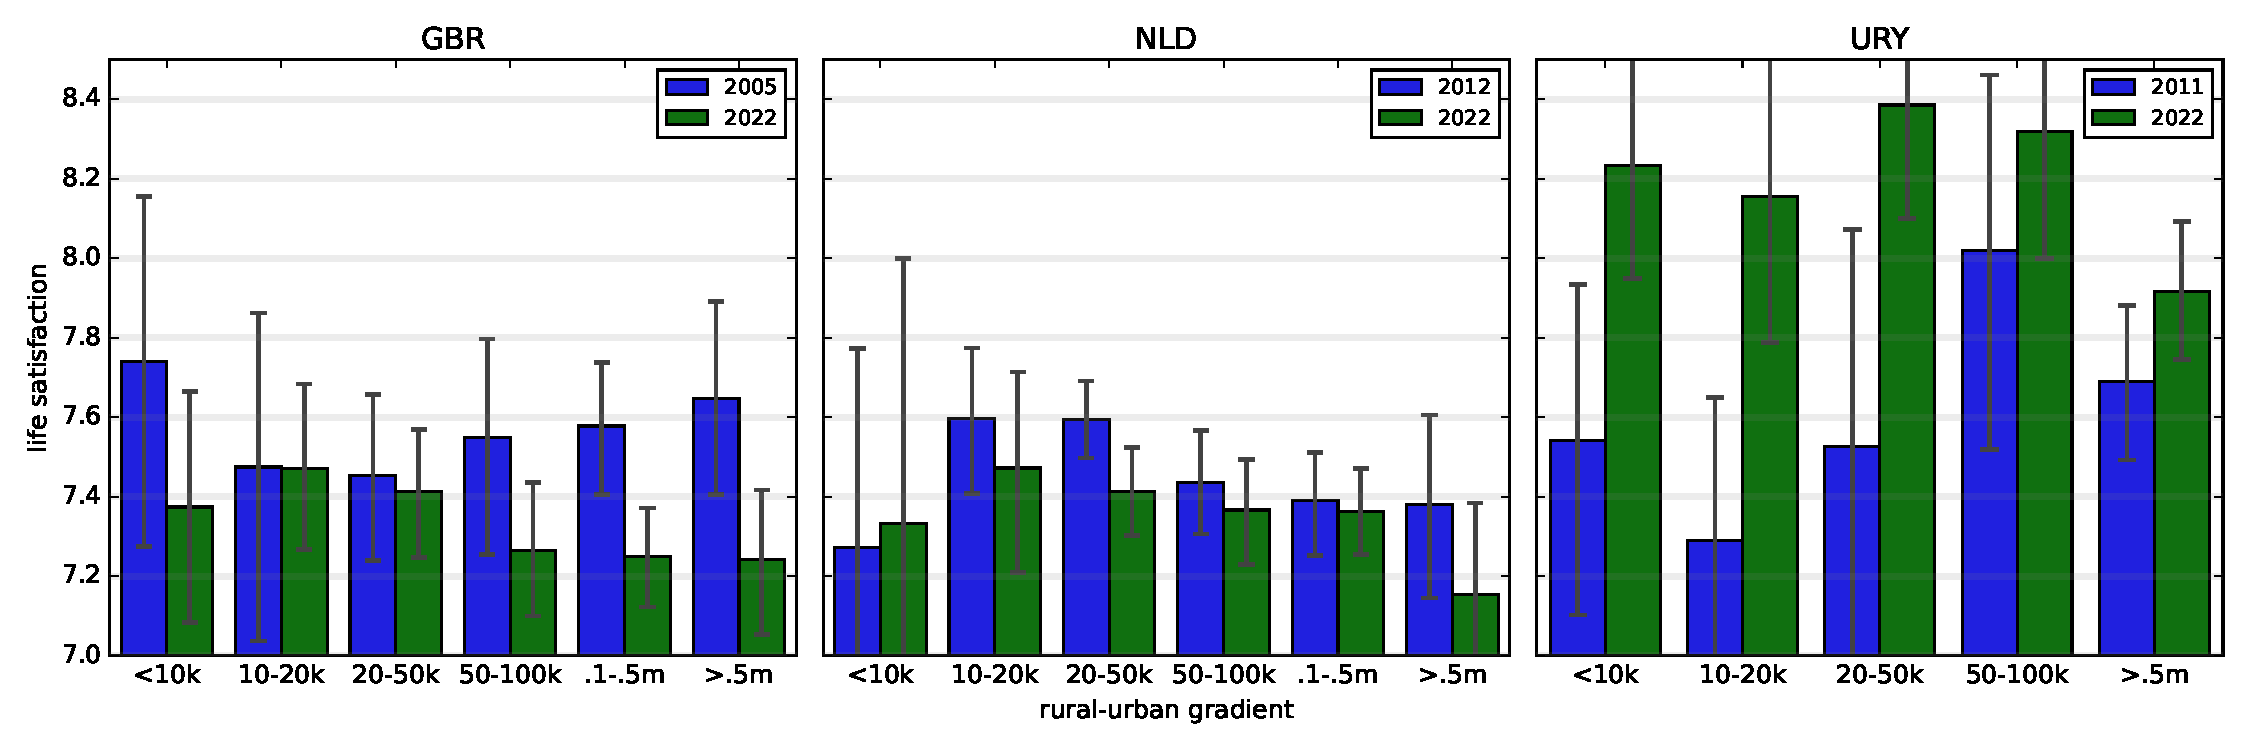
\includegraphics[height=3in]{bar.pdf}\centering\label{bar}
% \caption{Mean of life satisfaction and Eudaimonia by urbanicity.}
% \end{figure}
The OLS regressions\footnote{We use a standard OLS regression with robust
  standard errors, and treat the 11-step happiness variable as
  continuous. Ordinal logit and OLS regressions for ordinal  happiness data consistently yield similar results \citep{carbonell04}.
%                                                                                                                  
% OLS has become the default method in happiness research
% \citep{blanchflower11}. Theoretically, while there is still debate about the cardinality of SWB, there are strong arguments to treat it as a cardinal variable \citep{ng96,ng97}.
} of life satisfaction on urbanicity are shown in Table \ref{regA}.
 %
When interpreting these results, it is important to underscore that ecological
variables have relatively small effects on SWB as
 expected---most SWB is explained by genes \citep{schnittker08} and person level
 predictors \citep{veenhoven14b}. Nevertheless, the effect of urbanicity is
 about 0.5 on the 0-10 SWB scale,  which is similar to the
effect on SWB for adults when becoming unemployed \citep{clark2008lags}.
   
In columns a1-a3 % \footnote{Not in a4 controling for country dummies.}
there is a big difference in happiness between adolescents in the largest cities (gt1m) and smaller areas, consistent with previous research on adults \citep{aok-ls_fisher16}. But interestingly, unlike adults,
there is also a large gap between those who reside in places with less than 3k (reference category) and places with 3-15k people. This is especially evident in models a1-a3.% ; perhaps in the open country (lt3k) there are better outdoor play opportunities

Similar to research on adults \citep{aok21}, the addition of income/wealth makes
the results more pronounced---income/wealth confounds with urbanicity.
 %
In the full model, a4, we find that the urbanicity effect sizes remain large.

In models a4f and a4m, we split the analyses by gender and find that, urban unhappiness is higher for
females, a similar result to \citet{knight2010rural}: in rural China, men report lower happiness than women.

Model a5  adds the four internet usage variables  (% we postponed it to the last model because it
noting that this addition cuts the sample size by about 200k due to non-response),
and the results remain comparable.\footnote{In our 2018 dataset, internet use has very low correlation with urbanicity---see appendix for details.} % It probably has been the case
  % that internet was more of an urban phenomenon, but in an era of smartphones--internet is ubiquitious throught degrees of urbanness and
  % development levels.

%arthur
We investigate whether it may be that children in smaller places do not need as
much material wealth to be happy because they have other non-costly options for
entertainment. We test this by interacting the family wealth variable with the
urban/rural categories to see if the effect of material wealth on life
satisfaction differs according to place (hypothesizing a smaller effect of
family wealth in smaller places).
This happens to be the case in model a6, but once we add country dummies in
model a7, the effect disappears. 

\begin{table}[H]\centering\caption{OLS Regressions of Life Satisfaction. Base category for settlement size is $<$3k.} \label{regA} \begin{scriptsize} \begin{tabular}{p{1.6in}p{.5in}p{.5in}p{.5in}p{.5in}|p{.5in}p{.5in}|p{.5in}|p{.5in}p{.5in}p{.5 in}p{.5in}p{.5 in}}\hline                     &   $<.5m$   &     $>.5m$   &   $<.5m$   &     $>.5m$   &   URYrurTow   &     URYcity   \\
2022                &       -0.21** &       -0.41** &       -0.12** &       -0.23   &        0.75***&        0.23+  \\
constant            &        7.54***&        7.65***&        7.50***&        7.38***&        7.54***&        7.69***\\
N                   &        3111   &         521   &        3572   &         373   &        1154   &         836   \\
 \hline\multicolumn{4}{l}{*p$<$0.05 **p$<$0.01 ***p$<$0.001} \end{tabular}\end{scriptsize}\end{table}



Next, we run the full model, a4, for each country separately, with results
presented in Table \ref{a4cou} (note that results with sampling weights in the appendix
are similar). The table shows that in most countries adolescents are less happy
in cities ($>1m$) than in rural areas ($<3k$), except in Indonesia (IDN) and
Lebanon (LBN), where urbanites are happier than ruralites. {It is not uncommon in developing countries to observe greater
urban happiness since rural areas are often unlivable with insufficient availability of basic necessities such as food, water, and shelter.}%---better suffer urban disamenities than struggle to survive in a desert or jungle.   
 
The largest negative effect sizes, about -1, are in: the United Arab Emirates (ARE), Costa Rica (CRI), Russia (RUS), and Ukraine (UKR). 
 %
Future research could concentrate on the extremes and investigate what is it
about these specific countries that yield these large results. 

\begin{spacing}{.9} \begin{table}[H]\centering   \begin{scriptsize} \begin{tabular}{p{.5in}p{.5in}p{.5in}p{.5in}p{.5in}p{.5in}p{.5in}p{.5in}p{.5in}p{.5in}p{.5
                                                                      in}p{.5in}p{.5
                                                                      in}}\hline
                                                                      \input{a4couMOD.tex}
                                                                      \hline *
                                                                      p$<$0.05,
                                                                      $+$
                                                                      p$<$0.1;
                                                                      robust std
                                                                      err \end{tabular}\end{scriptsize}\caption{\label{a4cou}OLS
                                                                    Regressions
                                                                    of Life Satisfaction on
                                                                    place size
                                                                    for each
                                                                    country
                                                                    separately
                                                                    including
                                                                    covariates
                                                                    from a4 from
                                                                    table
                                                                    \ref{regA}. % Only
                                                                  % IDN and LBN
                                                                  % marginally
                                                                  % happier in
                                                                  % cities gt1m.
   Base category for settlement size is $<$3k.                                                               Results with sampling weights in appendix are similar.  
                                                           }\end{table} \end{spacing}



                                                       






\subsection*{Eudaimonia}

We turn to eudaimonia, a relatively rarely studied type of SWB. This particular measurement of happiness taps into a person's overall sense of satisfaction based on finding meaning in life. 

The results in Table \ref{regB} indicate an urban penalty of about 0.1-0.15 of a standard deviation in the largest cities ($>1m$).

 In Table \ref{regB}, the patterns observed are similar to those for life
 satisfaction: there is a large drop from less than 3k (lt3k) to 3-15k in models
 b1-b3, slightly less so
 in model b4 when controlling for country dummies. There is a clear gradient in
 models b4f and b4m. Females lose about twice the index points for eudaimonia
 than do males as urbanicity levels increase. 
 %
Controlling for internet use does not substantially change  the urbanicity
coefficients in model b5. % In model b6, wealth matters more in large cities. But in model b7, unexpectedly, we find that the effect of wealth matters less in large cities. We do not have an explanation for this result.
 We do not
have strong priors regarding the effect of family wealth on eudaimonia, but include the interaction results in
columns b6 and b7 for consistency with those for life satisfaction. From the results with country fixed effects
included, it appears that adolescents from richer families have an additional enhancement of eudaimonia in more
rural areas, a result worthy of further investigation.


\begin{table}[H]\centering\caption{OLS regressions of Eudaimonia. Base category for settlement size is $<$3k.} \label{regB} \begin{scriptsize} \begin{tabular}{p{1.6in}p{.5in}p{.5in}p{.5in}p{.5in}|p{.5in}p{.5in}|p{.5in}|p{.5in}p{.5in}p{.5 in}p{.5in}p{.5 in}}\hline                     &   $<.5m$   &     $>.5m$   &   $<.5m$   &     $>.5m$   &   URYrurTow   &     URYcity   \\
2022                &       -0.18*  &       -0.39+  &       -0.20***&       -0.45** &        0.42***&        0.21   \\
income              &        0.09***&        0.01   &        0.06***&        0.14***&        0.07*  &        0.13***\\
age                 &       -0.03*  &       -0.08** &       -0.02+  &       -0.06+  &        0.00   &       -0.06** \\
age2                &        0.00** &        0.00** &        0.00** &        0.00*  &       -0.00   &        0.00** \\
male                &       -0.18** &       -0.13   &       -0.11*  &       -0.27+  &        0.06   &        0.19   \\
married or living together as married&        0.53***&        0.74***&        0.44***&        0.23   &        0.46** &        0.06   \\
divorced/separated/widowed&        0.07   &        0.15   &       -0.11   &       -0.14   &       -0.37+  &       -0.19   \\
autonomy            &       -0.11*  &       -0.07   &       -0.11** &       -0.01   &       -0.06   &        0.06   \\
freedom             &        0.44***&        0.42***&        0.35***&        0.43***&        0.43***&        0.36***\\
trust               &        0.12+  &        0.42** &        0.43***&        0.28+  &       -0.05   &        0.10   \\
postmaterialist     &       -0.05   &       -0.18   &       -0.11*  &        0.14   &       -0.02   &        0.15   \\
god important       &        0.01   &        0.05*  &        0.02*  &       -0.01   &        0.05** &        0.06** \\
constant            &        4.08***&        5.95***&        4.59***&        4.80***&        3.47***&        4.58***\\
N                   &        1985   &         309   &        2283   &         237   &         736   &         579   \\
 \hline\multicolumn{4}{l}{*p$<$0.05 **p$<$0.01 ***p$<$0.001} \end{tabular}\end{scriptsize}\end{table}



In Table \ref{b4cou}, the urban eudaimonia penalty for large cities is a little less consistent than for the urban life satisfaction penalty. Nevertheless, the number of countries with a significant large city ($>$1m) penalty for
eudaimonia outweighs those with a significant large city premium by over 4:1. The weight of evidence is even
clearer for second tier cities (100k-1m) where the number of countries with a significant penalty outweighs those
with a significant premium by over 10:1.
% while adolescents in most countries experience an urban penalty, there is a handful
% with urban eudaimonic premium, especially in the Moscow region (QMR)\footnote{The Moscow Region (Russia) has degrees of urbanicity. % It is in addition to Russia.
% } at +.4. The countries were adolescents experience the largest penalty in eudaimonic happiness (of -.3 or
% more) are: the United Arab Emirates (ARE), Costa Rica (CRI), France (FRA), Korea, Rep. (KOR), Moldova (MDA), Baku (Azerbaijan (QAZ)), Tartarstan (Russia (QRT)), Russia (RUS) and Ukraine (UKR). Many of these countries overlap with those showing the lowest levels of life satisfaction in the previous section.  



\begin{spacing}{.9} \begin{table}[H]\centering   \begin{scriptsize} \begin{tabular}{p{.5in}p{.5in}p{.5in}p{.5in}p{.5in}p{.5in}p{.5in}p{.5in}p{.5in}p{.5in}p{.5
                                                                      in}p{.5in}p{.5
                                                                      in}}\hline
                                                                      \input{b4couMOD.tex}
                                                                      \hline *
                                                                      p$<$0.05,
                                                                      $+$
                                                                      p$<$0.1;
                                                                      robust std
                                                                      err \end{tabular}\end{scriptsize}\caption{\label{b4cou}OLS
                                                                    regressions
                                                                    of Eudaimonia on
                                                                    place size
                                                                    for each
                                                                    country
                                                                    separately
                                                                    including
                                                                    covariates
                                                                    from b4 (not
                                                                    shown). Base category for settlement size is $<$3k.  Most
                                                                    countries
                                                                    have 
                                                                    eudaimonic
                                                                    urban
                                                                    penalty, but
                                                                    a
                                                                    handful of
                                                                    countries
                                                                    have a 
                                                                    premium. See
                                                                    the appendix
                                                                    for results with sampling weights.% Results with sampling weights in appendix are weaker.
                                                           }\end{table} \end{spacing}





\section*{Conclusion and Discussion}
%Happiness may not be the ultimate goal for adults (e.g., duty, service, doing
%the right thing), but what else we want for the children and adolescents if not happiness.

The happiness literature is mainly focused on studying adults, with fewer studies focusing on children or adolescents. \citet{huebner2004research} offers some general observations on life
satisfaction in adolescents, and  others show that high life satisfaction in
adolescents is related to multiple beneficial outcomes
\citep{proctor2010very,suldo2006extremely}. A small number of happiness studies
use the PISA dataset% , for instance:
% \citet[][]{tang2019immigration,rudolf2020life,chung2021exploring,pan2023using}
% and \citet{marquez24}
.
Yet, there is no study focusing on urbanicity and how it affects happiness in adolescents. 

Our results provide  evidence that urban life is related to lower subjective
wellbeing of adolescents (measured both as life satisfaction and
eudaimonia). Although causality cannot be determined since this is an
observational study, these findings provide  support for previous research
involving adults % that was challenged by reverse causality arguments--
 especially given the lack of choice that teens have in deciding where to
 live. Our results suggest that there is something about city life, particularly
 in the largest cities,  that negatively impacts SWB. Urban unhappiness for
 adolescents is not due to any choice that they can make about moving to cities,
 rather it seems that cities' themselves, and their natural characteristics and
 problems (e.g., high density, high crime rate, high cost of living, too much
 stimuli and pollution)  affect adolescents' happiness.
 
Rurality, or smaller places, arguably provide more fertile ground for
spontaneity and freedom for young people---in rural areas kids can just go outside
and play, hang out and have fun without onerous rules and restrictions. Our finding that female adolescents experience a greater urban penalty than males may reflect
greater concern with crime and/or greater negative effects of inter-personal comparisons for females in an urban
relative to a more rural setting. % The setup, restrictions, and complexity of city life can weigh down on kids/teens.
The city is designed for  adults to work and to indulge in consumerism. Kids are
neither productive for jobs nor fit for many city amenities like airports,
universities, etc.\footnote{Of course, there are other amenities like some types
  of entertainment (theater, museums) that are fitting for kids, but cities
  weren't built with children/teens in mind. Schools in urban areas, for
  example, rarely have as much space for recreation as do rural schools.} 
%RV: I think we should remove the "elderly" angle and just focus on kids/teens
% Millions of people urbanize every year, most hoping to finding
% work.
% \footnote{The world's largest cities have the economic capacity and density
%   to produce stuff \citep{osullivan09}, just like in Engels' Manchester, where
%   capitalists used to crammed factory workers to produce without any regard for
%   their wellbeing, cities cram people closely together to extract as much
%   economic capital as possible. {``In a rather deep hole, in a curve
% of the Medlock and surrounded on all four sides by tall factories and high embankments, covered with
% buildings, stand two groups of about two hundred cottages, built chiefly back to back, in which live about four
% thousand human beings, most of them Irish. The cottages are old, dirty, and of the smallest sort, the streets
% uneven, fallen into ruts and in part without drains or pavement; masses of refuse, offal and sickening filth lie
% among standing pools in all directions; the atmosphere is poisoned by the effluvia from these, and laden and
% darkened by the smoke of a dozen tall factory chimneys. A horde of ragged women and children swarm about
% here, as filthy as the swine that thrive upon the garbage heaps and in the puddles. In short, the whole rookery
% furnishes such a hateful and repulsive spectacle as can hardly be equalled in the worst court on the Irk. The
% race that lives in these ruinous cottages, behind broken windows, mended with oilskin, sprung doors, and
% rotten door-posts, or in dark, wet cellars, in measureless filth and stench, in this atmosphere penned in as if
% with a purpose, this race must really have reached the lowest stage of
% humanity'' \citep{engels87}.}
% %Factories are largely gone to Asia, and what was is left of productive cities is office space. But COVID19 shook that up too. Perhaps, the main thing left is amenities like airports, hospitals, etc.
%  {Although what is mostly left of productive cities today in the West is office space since most factories have largely gone to Asia.}
% Wealth does matter a lot in the city---city life/experience is completely
% different for those at the top and those at the bottom of the economic
% ladder. Still, when accounting for country dummies, we did not find a
% differential positive effect of wealth in cities on life satisfaction, and if
% anything a  negative effect with eudaimonia. {Future research should explore this matter in depth to better make sense and explain these puzzling results.}}  

One explanation as to why rural kids may be happier is that their parents are
happier and this flows through to their offspring (which is a type of  selection
effect). However, the prior research cited earlier indicates that the link between parent and child wellbeing may
be quite weak. Furthermore, our results show a large gap in adolescent wellbeing between places with fewer than 3k
people and places with 3-15k people.
 In contrast, the literature does not indicate any such gap for adults. Hence,
selection on adult wellbeing does not appear to explain the adolescent wellbeing gradient for
urbanicity.

% , contradicting this explanation to some
% degree--a useful result for robustness.
% % RV: maybe we need to add a bit more on this point, how does this contract to some extent the argument, not entirely sure to me
% % rubia
% An important
One limitation is that although we would like to take into account possible grandparents and siblings effects, we do not have such measures in the 2018 PISA. % also look into the caretakers and extended family (grandparents).
In cities, many live with their nuclear family, far away from relatives and both
parents usually work leaving their kids in the  care of others, so urban parents
may spend less time with their kids than those in rural areas. In smaller
places, care-giving may be
more commonly conducted by parents, grandparents or other extended relatives, contributing to happiness. 
Future research should ideally also  control for the number of siblings
especially given that people in smaller places and rural areas still have more kids than people living in mega-cities \citep{lerch2019regional}. % Kids having other kids around to interact and play with can boost happiness. Finally, arguably after the pandemic, adolescents in cities became even more unhappy just as adults did
% \textbf{$<<blind for peer-review>>$}. 
%RV: should we simply just add the citation above and remove blind for peer-review? we cite ourselves already a lot lol...
%aok this one will have to pupdate anyway, its unpublished now hopefully will be
%published soon
\section*{Takeaways for Practice}

%We all want happiness for the children and adolescents. 

These findings should be of interest to policymakers, administrators, schools, and particularly to parents. Most parents want their children to be happy and these results suggest that where they choose to settle to start a family matters---to achieve greater happiness for their kids they should enjoy more rurality and nature. 

Cities are  for adults---to work, produce, and consume. Much of  the production-related built environment such as factories and offices is irrelevant for children and adolescents. % Transportation networks such as roads and railways
% are dangerous for little ones. And
 So too is much of the consumption-related built environment  such as
 nightclubs, higher education, most healthcare and many stores. 

Research on urbanicity and subjective well-being is crucial as it sparks
conversations about how to lead a happier life. It also empowers individuals to
make life-altering decisions, such as choosing where to live and raise a
family. At the same time, for income-generation reasons, advocating for living
in smaller areas is  problematic. Thus, we are not suggesting that young
families should flock to rural areas. We are simply highlighting what is lost and suggesting that urban parents and caregivers should try to expose their children to more rurality, for instance by organizing
trips, vacations and other activities outside of cities. Through such avenues,
urban kids can enjoy at least a taste of rural life. 


                                                       
% %table centered on decimal points:)
% \begin{table}[H]\centering\footnotesize
% \caption{\label{freq_im_god} importance of God}
% \begin{tabular} {@{} lrrrr @{}}   \hline 
% Item& Number & Per cent   \\ \hline
% 1(not at all)&    9,285&  9\\
% 2&    3,555&        3\\
% 3&    3,937&        4\\
% 4&    2,888&        3\\
% 5&    7,519&        7\\
% 6&    5,175&        5\\
% 7&    6,050&        6\\
% 8&    8,067&        8\\
% 9&    8,463&        8\\
% 10&   52,385&       49\\
% Total&  107,324&      100\\ \hline
% \end{tabular}\end{table}


% % Define block styles
% \tikzstyle{block} = [rectangle, draw, fill=black!20, 
%     text width=10em, text centered, rounded corners, minimum height=4em]
% \tikzstyle{b} = [rectangle, draw,  
%     text width=6em, text centered, rounded corners, minimum height=4em]
% \tikzstyle{line} = [draw, -latex']
% \tikzstyle{cloud} = [draw, ellipse,fill=black!20, node distance = 5cm,
%     minimum height=2em]
    
% \begin{tikzpicture}[node distance = 2cm, auto]
%     % Place nodes
%     \node [block] (lib) {liberalism, egalitarianism, welfare};
%     \node [block, below of=lib] (con) {conservatism, competition, individualism};
%     \node [cloud, right of=con] (ls) {well-being};
%     \node [block, below of=ls] (cul) {genes, culture};
%     \node [b, left of =lib, node distance = 4cm] (c) {country-level};
%     \node [b, left of =con,  node distance = 4cm] (c) {person-level};
%     % Draw edges
%     \path [line] (lib) -- (ls);
%     \path [line] (con) -- (ls);
%     \path [line,dashed] (cul) -- (ls);
% \end{tikzpicture}


%PUT THIS NOTE, polish and put to /root/author_what_data --ALWAYS
%stick here stuff as i run it!!! maybe comment out later...


% TODO: have separate som-r.tex as opposed to having it below; and in paper say
% see supplemetary material as opposed to see appendix!

%\newpage
%\theendnotes
\bibliography{/home/aok/papers/root/tex/ebib.bib,/home/aok/papers/root/old/2022/swbUrbRurPsid/tex/swbUrbRurPsid.bib,pisa.bib,references.bib}


 \section*{\Huge ONLINE APPENDIX}
 \textbf{[note: this section will NOT be a part of the final version of
   the manuscript, but will be available online instead]} %hence everything below
                                 %is organized byu section, not subsection
% !!!
% have most of the stuff outputted to online appendix:)--start with that and then
% select stuff to paper--have brief narrative describng patterns in online app too
% !!!

% \section*{Variables' definitions, coding, and distributions}
% \label{app_var_des}




\section{Additional Results}

\input{h1.tex}

\begin{spacing}{.9} \begin{table}[H]\centering   \begin{scriptsize} \begin{tabular}{p{.5in}p{.5in}p{.5in}p{.5in}p{.5in}p{.5in}p{.5in}p{.5in}p{.5in}p{.5in}p{.5
                                                                      in}p{.5in}p{.5
                                                                      in}}\hline
                                                                      \input{../out/a1.tex}
                                                                      \hline *
                                                                      p$<$0.05,
                                                                      $+$
                                                                      p$<$0.1;
                                                                      robust std
                                                                      err \end{tabular}\end{scriptsize}\caption{\label{d1}OLS
                                                                    regressions
                                                                    of SWB on
                                                                    place size
                                                                    only
                                                                    (bivariate; a1)
                                                                    for each
                                                                    country
                                                                    separately. Base category for settlement size is $<$3k.
                                                                  }\end{table} \end{spacing}


\section{internet use}

Urbanicity has very low positive correlation with internet use

\begin{spacing}{.5}
\begin{scriptsize}
\begin{verbatim}
. d city int*

Variable      Storage   Display    Value
    name         type    format    label      Variable label
-------------------------------------------------------------------------------
city            byte    %9.0g      city       RECODE of SC001Q01TA (Which of
                                                the following definitions best
                                                describes the comm
intWday         byte    %2.0f      labels341
                                              During a typical weekday, for how
                                                long do you use the Internet
                                                outside of school
intWend         byte    %2.0f      labels342
                                              On a typical weekend day, for how
                                                long do you use the Internet
                                                outside of school
intSN           byte    %2.0f      labels374
                                              Use digital devices outside of
                                                school: Participating in Social
                                                Networks (e.g. <F
intFun          byte    %2.0f      labels376
                                              Use digital devices outside of
                                                school: Browsing the Internet
                                                for fun (such as wa


. pwcorr city int*

             |     city  intWday  intWend    intSN   intFun
-------------+---------------------------------------------
        city |   1.0000 
     intWday |   0.0488   1.0000 
     intWend |   0.0720   0.7251   1.0000 
       intSN |   0.0569   0.2594   0.2792   1.0000 
      intFun |   0.0866   0.3066   0.3479   0.5249   1.0000 
\end{verbatim}
\end{scriptsize}
\end{spacing}{.9}

Using some internet is good for an adolescent, but using a lot on the weekend is bad


\begin{spacing}{.5}
\begin{scriptsize}
\begin{verbatim}
reg ls i.city wealth fem faEd i.intWday i.intWend, robust

Linear regression                               Number of obs     =    266,770
                                                F(19, 266750)     =     340.73
                                                Prob > F          =     0.0000
                                                R-squared         =     0.0238
                                                Root MSE          =     2.5032

------------------------------------------------------------------------------
             |               Robust
          ls | Coefficient  std. err.      t    P>|t|     [95% conf. interval]
-------------+----------------------------------------------------------------
        city |
      3-15k  |  -.4296694   .0196451   -21.87   0.000    -.4681732   -.3911656
    15-100k  |  -.4853962   .0185923   -26.11   0.000    -.5218366   -.4489557
    100k-1m  |  -.5295389   .0186871   -28.34   0.000    -.5661651   -.4929126
       gt1m  |  -.7087667   .0212434   -33.36   0.000    -.7504032   -.6671301
             |
      wealth |    .058285   .0053595    10.87   0.000     .0477805    .0687896
         fem |  -.4855582   .0097124   -49.99   0.000    -.5045942   -.4665223
        faEd |  -.0238479   .0051004    -4.68   0.000    -.0338445   -.0138513
             |
     intWday |
1-30 minu..  |   .1687749   .0381252     4.43   0.000     .0940505    .2434993
31-60 min..  |   .1174412   .0369693     3.18   0.001     .0449823    .1899001
Between 1..  |   .0837295   .0347786     2.41   0.016     .0155643    .1518946
Between 2..  |  -.0017767   .0345739    -0.05   0.959    -.0695406    .0659872
Between 4..  |  -.0369376   .0357303    -1.03   0.301    -.1069681    .0330928
More than..  |   .0083298   .0365747     0.23   0.820    -.0633557    .0800153
             |
     intWend |
1-30 minu..  |    .241415    .046509     5.19   0.000     .1502586    .3325714
31-60 min..  |    .296678   .0448001     6.62   0.000     .2088711     .384485
Between 1..  |   .2990314    .042022     7.12   0.000     .2166694    .3813934
Between 2..  |      .1492   .0414603     3.60   0.000     .0679389     .230461
Between 4..  |  -.0009641   .0418857    -0.02   0.982     -.083059    .0811307
More than..  |  -.2383889   .0423359    -5.63   0.000    -.3213662   -.1554117
             |
       _cons |   7.966607   .0429739   185.38   0.000     7.882379    8.050834
------------------------------------------------------------------------------
\end{verbatim}
\end{scriptsize}
\end{spacing}{.9}



And below another robustness check, using clustered std err on school and school
level covariates--results similar
\begin{spacing}{.5}
\begin{scriptsize}
\begin{verbatim}

. d STRATIO SCHLTYPE CLSIZE EDUSHORT STAFFSHORT STUBEHA TEACHBEHA 

Variable      Storage   Display    Value
    name         type    format    label      Variable label
------------------------------------------------------------------------------
STRATIO         double  %10.0g                Student-Teacher ratio
SCHLTYPE        byte    %10.0g                School Ownership
CLSIZE          byte    %10.0g                Class Size
EDUSHORT        double  %10.0g                Shortage of educational material
                                                (WLE)
STAFFSHORT      double  %10.0g                Shortage of educational staff
                                                (WLE)
STUBEHA         double  %10.0g                Student behaviour hindering
                                                learning (WLE)
TEACHBEHA       double  %10.0g                Teacher behaviour hindering
                                                learning (WLE)


. reg ls i.city wealth i.gender faEd i.Region STRATIO SCHLTYPE CLSIZE EDUSHORT
>  STAFFSHORT STUBEHA TEACHBEHA , robust cluster(CNTSCHID)

Linear regression                               Number of obs     =    389,098
                                                F(131, 15010)     =     129.21
                                                Prob > F          =     0.0000
                                                R-squared         =     0.0686
                                                Root MSE          =      2.488

                          (Std. err. adjusted for 15,011 clusters in CNTSCHID)
------------------------------------------------------------------------------
             |               Robust
          ls | Coefficient  std. err.      t    P>|t|     [95% conf. interval]
-------------+----------------------------------------------------------------
        city |
      3-15k  |      -0.19       0.02    -8.07    0.00        -0.24       -0.14
    15-100k  |      -0.26       0.02   -11.18    0.00        -0.31       -0.22
    100k-1m  |      -0.41       0.02   -16.91    0.00        -0.45       -0.36
       gt1m  |      -0.44       0.03   -16.02    0.00        -0.49       -0.38
             |
      wealth |       0.21       0.01    38.32    0.00         0.20        0.22
             |
      gender |
       Male  |       0.40       0.01    42.56    0.00         0.38        0.42
        faEd |      -0.02       0.00    -5.15    0.00        -0.03       -0.01
             |
      Region | -----COUNTRY DUMMIES OMITTED HERE---------
             |
     STRATIO |       0.00       0.00     0.71    0.48        -0.00        0.00
    SCHLTYPE |       0.06       0.01     5.75    0.00         0.04        0.09
      CLSIZE |       0.00       0.00     2.39    0.02         0.00        0.00
    EDUSHORT |       0.01       0.01     2.07    0.04         0.00        0.03
  STAFFSHORT |      -0.01       0.01    -1.07    0.29        -0.02        0.01
     STUBEHA |       0.01       0.01     1.15    0.25        -0.01        0.02
   TEACHBEHA |      -0.02       0.01    -2.34    0.02        -0.03       -0.00
       _cons |       8.66       0.07   117.75    0.00         8.52        8.81
------------------------------------------------------------------------------




\end{verbatim}
\end{scriptsize}
\end{spacing}{.9}

Finally sampling weights--results similar for life satisfaction, but weaker for
 eudaimonia. Also see
\url{https://www.statalist.org/forums/forum/general-stata-discussion/general/1435058-should-i-apply-weights-when-i-use-the-tabulate-command-oecd-pisa-analysis}
and \url{https://largescaleassessmentsineducation.springeropen.com/articles/10.1186/s40536-021-00099-0}

\begin{spacing}{.5}
\begin{scriptsize}
\begin{verbatim}

. reg ls i.city, robust  //it is huuuge yay!

Linear regression                               Number of obs     =    471,551
                                                F(4, 471546)      =     398.44
                                                Prob > F          =     0.0000
                                                R-squared         =     0.0034
                                                Root MSE          =     2.5877

------------------------------------------------------------------------------
             |               Robust
          ls | Coefficient  std. err.      t    P>|t|     [95% conf. interval]
-------------+----------------------------------------------------------------
        city |
      3-15k  |      -0.34       0.01   -23.16    0.00        -0.37       -0.32
    15-100k  |      -0.37       0.01   -26.19    0.00        -0.40       -0.34
    100k-1m  |      -0.44       0.01   -30.78    0.00        -0.47       -0.41
       gt1m  |      -0.61       0.02   -38.86    0.00        -0.64       -0.58
             |
       _cons |       7.63       0.01   624.06    0.00         7.61        7.66
------------------------------------------------------------------------------

. 
end of do-file

. do "/tmp/SD17808.000000"

. reg ls i.city [pw=W_FSTUWT], robust 
(sum of wgt is 24,137,093.50498)

Linear regression                               Number of obs     =    471,551
                                                F(4, 471546)      =     107.54
                                                Prob > F          =     0.0000
                                                R-squared         =     0.0060
                                                Root MSE          =      2.611

------------------------------------------------------------------------------
             |               Robust
          ls | Coefficient  std. err.      t    P>|t|     [95% conf. interval]
-------------+----------------------------------------------------------------
        city |
      3-15k  |      -0.31       0.04    -7.59    0.00        -0.39       -0.23
    15-100k  |      -0.48       0.04   -13.33    0.00        -0.56       -0.41
    100k-1m  |      -0.61       0.04   -16.85    0.00        -0.68       -0.54
       gt1m  |      -0.68       0.04   -18.14    0.00        -0.76       -0.61
             |
       _cons |       7.57       0.03   235.80    0.00         7.51        7.64
------------------------------------------------------------------------------

. 
end of do-file

. do "/tmp/SD17808.000000"

. reg ls i.city wealth fem faEd i.Region, robust beta 

Linear regression                               Number of obs     =    452,931
                                                F(128, 452802)    =     299.51
                                                Prob > F          =     0.0000
                                                R-squared         =     0.0697
                                                Root MSE          =     2.4886

------------------------------------------------------------------------------
             |               Robust
          ls | Coefficient  std. err.      t    P>|t|                     Beta
-------------+----------------------------------------------------------------
        city |
      3-15k  |      -0.19       0.02   -12.48    0.00                    -0.03
    15-100k  |      -0.25       0.01   -17.35    0.00                    -0.04
    100k-1m  |      -0.40       0.01   -27.55    0.00                    -0.07
       gt1m  |      -0.46       0.02   -26.97    0.00                    -0.06
             |
      wealth |       0.21       0.00    48.55    0.00                     0.10
         fem |      -0.39       0.01   -52.08    0.00                    -0.07
        faEd |      -0.02       0.00    -5.06    0.00                    -0.01
             |
      Region | -----COUNTRY DUMMIES OMITTED HERE-----
       _cons |       9.34       0.03   305.46    0.00                        .
------------------------------------------------------------------------------

. 
end of do-file

. do "/tmp/SD17808.000000"

. reg ls i.city wealth fem faEd i.Region [pw=W_FSTUWT], robust
(sum of wgt is 23,248,792.65115)

Linear regression                               Number of obs     =    452,931
                                                F(128, 452802)    =     252.32
                                                Prob > F          =     0.0000
                                                R-squared         =     0.0587
                                                Root MSE          =     2.5304

------------------------------------------------------------------------------
             |               Robust
          ls | Coefficient  std. err.      t    P>|t|     [95% conf. interval]
-------------+----------------------------------------------------------------
        city |
      3-15k  |      -0.22       0.04    -5.04    0.00        -0.30       -0.13
    15-100k  |      -0.30       0.04    -7.60    0.00        -0.37       -0.22
    100k-1m  |      -0.46       0.04   -11.93    0.00        -0.54       -0.38
       gt1m  |      -0.45       0.04   -10.95    0.00        -0.53       -0.37
             |
      wealth |       0.18       0.01    17.53    0.00         0.16        0.20
         fem |      -0.32       0.02   -17.08    0.00        -0.36       -0.28
        faEd |      -0.00       0.01    -0.13    0.90        -0.02        0.02
             |
      Region |-----COUNTRY DUMMIES OMITTED HERE-----
       _cons |       9.27       0.05   198.36    0.00         9.18        9.37
------------------------------------------------------------------------------

. 
end of do-file

. do "/tmp/SD17808.000000"

. reg EUDMO i.city, robust  

Linear regression                               Number of obs     =    483,844
                                                F(4, 483839)      =     242.03
                                                Prob > F          =     0.0000
                                                R-squared         =     0.0019
                                                Root MSE          =     .97663

------------------------------------------------------------------------------
             |               Robust
       EUDMO | Coefficient  std. err.      t    P>|t|     [95% conf. interval]
-------------+----------------------------------------------------------------
        city |
      3-15k  |      -0.09       0.01   -16.55    0.00        -0.10       -0.08
    15-100k  |      -0.13       0.01   -25.09    0.00        -0.14       -0.12
    100k-1m  |      -0.14       0.01   -27.48    0.00        -0.15       -0.13
       gt1m  |      -0.15       0.01   -26.23    0.00        -0.16       -0.14
             |
       _cons |       0.27       0.00    61.12    0.00         0.26        0.28
------------------------------------------------------------------------------

. 
end of do-file

. do "/tmp/SD17808.000000"

. reg EUDMO i.city [pw=W_FSTUWT], robust  
(sum of wgt is 24,302,689.2416)

Linear regression                               Number of obs     =    483,844
                                                F(4, 483839)      =     121.94
                                                Prob > F          =     0.0000
                                                R-squared         =     0.0062
                                                Root MSE          =       .955

------------------------------------------------------------------------------
             |               Robust
       EUDMO | Coefficient  std. err.      t    P>|t|     [95% conf. interval]
-------------+----------------------------------------------------------------
        city |
      3-15k  |      -0.07       0.01    -5.04    0.00        -0.09       -0.04
    15-100k  |      -0.17       0.01   -14.08    0.00        -0.20       -0.15
    100k-1m  |      -0.22       0.01   -17.58    0.00        -0.24       -0.19
       gt1m  |      -0.21       0.01   -16.79    0.00        -0.24       -0.19
             |
       _cons |       0.35       0.01    33.16    0.00         0.33        0.37
------------------------------------------------------------------------------

. 
end of do-file

. do "/tmp/SD17808.000000"

. reg EUDMO i.city wealth fem faEd i.Region, robust beta 

Linear regression                               Number of obs     =    465,568
                                                F(131, 465436)    =     226.40
                                                Prob > F          =     0.0000
                                                R-squared         =     0.0575
                                                Root MSE          =     .94722

------------------------------------------------------------------------------
             |               Robust
       EUDMO | Coefficient  std. err.      t    P>|t|                     Beta
-------------+----------------------------------------------------------------
        city |
      3-15k  |      -0.05       0.01    -8.25    0.00                    -0.02
    15-100k  |      -0.06       0.01   -11.49    0.00                    -0.03
    100k-1m  |      -0.10       0.01   -19.37    0.00                    -0.05
       gt1m  |      -0.13       0.01   -20.65    0.00                    -0.05
             |
      wealth |       0.06       0.00    36.44    0.00                     0.07
         fem |      -0.07       0.00   -24.54    0.00                    -0.03
        faEd |       0.01       0.00     4.07    0.00                     0.01
             |
      Region |-----COUNTRY DUMMIES OMITTED HERE-----
       _cons |       0.74       0.01    58.53    0.00                        .
------------------------------------------------------------------------------

. 
end of do-file

. do "/tmp/SD17808.000000"

. reg EUDMO i.city wealth fem faEd i.Region [pw=W_FSTUWT], robust
(sum of wgt is 23,464,999.88423)

Linear regression                               Number of obs     =    465,568
                                                F(131, 465436)    =     179.18
                                                Prob > F          =     0.0000
                                                R-squared         =     0.0696
                                                Root MSE          =     .92214

------------------------------------------------------------------------------
             |               Robust
       EUDMO | Coefficient  std. err.      t    P>|t|     [95% conf. interval]
-------------+----------------------------------------------------------------
        city |
      3-15k  |      -0.02       0.01    -1.29    0.20        -0.05        0.01
    15-100k  |      -0.03       0.01    -2.41    0.02        -0.06       -0.01
    100k-1m  |      -0.07       0.01    -5.14    0.00        -0.09       -0.04
       gt1m  |      -0.06       0.01    -4.04    0.00        -0.09       -0.03
             |
      wealth |       0.04       0.00    10.86    0.00         0.03        0.05
         fem |      -0.04       0.01    -5.29    0.00        -0.05       -0.02
        faEd |       0.01       0.00     1.66    0.10        -0.00        0.01
             |
      Region |-----COUNTRY DUMMIES OMITTED HERE-----
       _cons |       0.69       0.02    39.15    0.00         0.65        0.72
------------------------------------------------------------------------------

. 
end of do-file

. do "/tmp/SD17808.000000"

. reg EUDMO i.city wealth fem faEd i.Region, robust beta 

Linear regression                               Number of obs     =    465,568
                                                F(131, 465436)    =     226.40
                                                Prob > F          =     0.0000
                                                R-squared         =     0.0575
                                                Root MSE          =     .94722

------------------------------------------------------------------------------
             |               Robust
       EUDMO | Coefficient  std. err.      t    P>|t|                     Beta
-------------+----------------------------------------------------------------
        city |
      3-15k  |      -0.05       0.01    -8.25    0.00                    -0.02
    15-100k  |      -0.06       0.01   -11.49    0.00                    -0.03
    100k-1m  |      -0.10       0.01   -19.37    0.00                    -0.05
       gt1m  |      -0.13       0.01   -20.65    0.00                    -0.05
             |
      wealth |       0.06       0.00    36.44    0.00                     0.07
         fem |      -0.07       0.00   -24.54    0.00                    -0.03
        faEd |       0.01       0.00     4.07    0.00                     0.01
             |
      Region |-----COUNTRY DUMMIES OMITTED HERE-----
       _cons |       0.74       0.01    58.53    0.00                        .
------------------------------------------------------------------------------

. 
end of do-file

. 

\end{verbatim}
\end{scriptsize}
\end{spacing}{.9}



% %\input{/tmp/a.tex} %aok_var_des

% % \begin{spacing}{.9}
% %   \begin{table}[H]\centering \caption{Summary statistics.} \label{sumSta} \begin{scriptsize} \begin{tabular}{p{1.8in}p{.5in}p{.5in}p{.5in}p{.5in}p{.5in}p{.5in}p{.5in}p{.5in}p{.5in}p{.5
% %             in}p{.5in}p{.5 in}}\hline
% %         \input{/tmp/aha2.tex}
% %          \end{tabular}\end{scriptsize}\end{table}
% % \end{spacing}

% % \begin{spacing}{.9}
% %   \begin{table}[H]\centering \caption{Correlation matrix.} \label{sumSta} \begin{scriptsize} \begin{tabular}{@{}
% %           p{1.2in} rrrrrrrrrrrrr @{}}\hline
% %         \input{/tmp/ahb2.tex}\hline
% %          \end{tabular}\end{scriptsize}\end{table}
% % \end{spacing}



% Table XXX shows variable distributions. If a variable has more than
% 10 categories it is classified into bins...

% %\input .... %TODO !!!! have input here histograms

% \section*{Additional Descriptive Statistics}
% \label{app_des_sta}

% %make sure i have [H] or h! ???
% % \begin{table}[H]
% % \caption{}
% % \centering
% % \label{}
% % \begin{scriptsize}
% % \input{../out/reg_c.tex}
% % \end{scriptsize}
% % \end{table}


\end{spacing}
\end{document}
